\clearpage
\onecolumn
\appendix
\setcounter{secnumdepth}{2}

\section{Additional Cross-Dataset Diagnostics}
\label{app:auto-completed}
% BEGIN AUTO_RESULTS
We report completed, protocol-matched diagnostics on the two Amazon datasets used in the main paper. These results assess the robustness of our TIGER-style implementation; they are not presented as reproductions of the published TIGER architecture.
\begin{table}[H]
\centering
\small
\begin{tabular}{llrrrrr}
\toprule
Dataset & Seed & R@10 & N@10 & R@30 & R@90 & TargetInOutput@100 \\
\midrule
Beauty & 42 & 0.0464 & 0.0262 & 0.0823 & 0.1392 & 14.55\% \\
Beauty & 43 & 0.0443 & 0.0261 & 0.0766 & 0.1299 & 13.71\% \\
Beauty & 44 & 0.0525 & 0.0295 & 0.0945 & 0.1568 & 16.40\% \\
Sports & 42 & 0.0205 & 0.0109 & 0.0418 & 0.0834 & 8.87\% \\
Sports & 43 & 0.0242 & 0.0126 & 0.0509 & 0.1015 & 10.80\% \\
Sports & 44 & 0.0261 & 0.0135 & 0.0543 & 0.1066 & 11.39\% \\
\bottomrule
\end{tabular}
\caption{TIGER-style SID diagnostics under constrained-validation checkpoint
selection and valid-prefix decoding. Beauty and Sports use 22,363 and 21,519
test users, respectively; every row uses exactly 100 valid, distinct,
history-filtered items for TargetInOutput@100.}
\label{tab:auto-tiger-results}
\end{table}

\section{Training-Seed Stability}
\label{app:seed-stability}

Table~\ref{tab:ml1m-seven-seed} reports every completed ML-1M training seed
under the final common protocol. TIGER uses valid-prefix constrained decoding,
exact code lookup, and adaptive internal over-generation. Its mean
TargetInOutput is \(0.6667\pm0.0018\) at an effective returned-list size of
100 and \(0.7593\pm0.0025\) at size 200. Across seven seeds, the 95\% $t$
intervals for R@10 are $[0.2930,0.3063]$ for TIGER,
$[0.3060,0.3147]$ for CQG-Single, and $[0.2947,0.3006]$ for CQG-AR.
CQG-Single exceeds TIGER in all seven indexed runs. The mean paired
seed-level R@10 difference is 0.0107 (95\% paired $t$ interval
[0.0021, 0.0193]); an exact two-sided sign-flip permutation test over the
seven paired differences gives $p=.0156$. These intervals quantify
training-seed variation; they are distinct from the paired seed-42 user
bootstrap in Appendix~\ref{app:crossover-values}.

All three methods use the same frozen SASRec item-embedding table, processed
split, and evaluation
history. For CQG-Single and CQG-AR, seeds 42--48 change downstream-model
initialization, minibatch order, and stochastic optimization while leaving the
item table fixed. For TIGER, the same indexed seed also changes hierarchical
$k$-means initialization and SID-decoder training. Thus ``paired seed''
denotes matched replicate indices under a common item space and protocol; it
does not imply that the three architectures consume identical random draws.

\begin{table}[H]
\centering
\small
\setlength{\tabcolsep}{5pt}
\begin{tabular}{lrrrrrr}
\toprule
Seed & \multicolumn{2}{c}{TIGER} & \multicolumn{2}{c}{CQG-Single} &
\multicolumn{2}{c}{CQG-AR} \\
\cmidrule(lr){2-3}\cmidrule(lr){4-5}\cmidrule(lr){6-7}
& R@10 & N@10 & R@10 & N@10 & R@10 & N@10 \\
\midrule
42 & 0.2992 & 0.1756 & 0.3036 & 0.1736 & 0.2972 & 0.1720 \\
43 & 0.3038 & 0.1751 & 0.3161 & 0.1874 & 0.3028 & 0.1750 \\
44 & 0.2841 & 0.1644 & 0.3144 & 0.1831 & 0.2945 & 0.1711 \\
45 & 0.3028 & 0.1768 & 0.3103 & 0.1830 & 0.3010 & 0.1755 \\
46 & 0.3045 & 0.1781 & 0.3139 & 0.1849 & 0.2969 & 0.1739 \\
47 & 0.2995 & 0.1728 & 0.3089 & 0.1832 & 0.2970 & 0.1734 \\
48 & 0.3036 & 0.1747 & 0.3053 & 0.1804 & 0.2940 & 0.1738 \\
\midrule
Mean & 0.2996 & 0.1739 & \textbf{0.3104} & \textbf{0.1822} & 0.2976 & 0.1735 \\
Sample SD & 0.0072 & 0.0046 & 0.0047 & 0.0044 & 0.0032 & 0.0016 \\
\bottomrule
\end{tabular}
\caption{Seven-seed ML-1M results under valid-prefix constrained TIGER
decoding. Each TIGER row uses the checkpoint reselected by constrained
validation and evaluates all 6,040 test users with the same history filtering.
N@10 denotes NDCG@10.}
\label{tab:ml1m-seven-seed}
\end{table}

\paragraph{Preliminary Sports multimodal diagnostic.}
We additionally ran a single-seed diagnostic in which CQG-Single, CQG-AR, and the TIGER-style decoder share item embeddings formed from collaborative features and ImageNet-pretrained ResNet-18 image features. Images were available for only 5,268 of 10,693 non-padding catalog items; items without an image use the collaborative component with a zero image feature. Because image availability is incomplete and no multi-seed estimate is available, this experiment is preliminary and is not used to support the main claims.
\begin{table}[H]
\centering
\small
\begin{tabular}{lrrrr}
\toprule
Method & R@10 & NDCG@10 & R@90 & TargetInOutput@100 \\
\midrule
CQG-Single (multimodal, seed 42) & 0.0326 & 0.0174 & 0.1154 & -- \\
CQG-AR (multimodal, seed 42) & 0.0296 & 0.0161 & 0.1087 & 11.62\% \\
TIGER-style SID (multimodal, seed 42) & 0.0254 & 0.0137 & 0.0972 & 10.06\% \\
\bottomrule
\end{tabular}
\caption{Preliminary single-seed Sports multimodal diagnostic. CQG-Single,
CQG-AR, and the TIGER-style SID model use the same fused item space; the result
is not directly comparable to a full-coverage multimodal benchmark because only
49.3\% of catalog items have images.}
\label{tab:auto-sports-mm}
\end{table}

% END AUTO_RESULTS

\section{Experimental Protocol and Reproducibility}
\label{app:protocol}

\subsection{MSE-Trained Retrieve-and-Rerank Diagnostics}
\label{app:mse-rerank}

We evaluate a matched 100-candidate retrieve-and-rerank pipeline using
MSE-trained continuous-query checkpoints. Across ML-1M, Beauty, and Sports,
CQG-Single followed by SASRec reranking reaches 97.7--102\% of full-rank
SASRec Recall@10; the completed CQG-AR controls on Beauty and Sports are also
reported in Table~\ref{tab:cross}. Table~\ref{tab:hierarchy} further
compares the learned retriever with random, last-item kNN, and mean-of-five
kNN baselines under the same SASRec reranker. These candidate-generation
diagnostics are separate from the CE-trained standalone results in
Table~\ref{tab:primary-comparison}.

\begin{table}[H]
\centering
\small
\begin{tabular}{lrrr}
\toprule
Method & ML-1M & Beauty & Sports \\
\midrule
\multicolumn{4}{l}{\textit{Recall@10}} \\
SASRec & 0.2797 & 0.0558 & 0.0390 \\
CQG-Single MSE standalone & 0.2425 & 0.0524 & 0.0307 \\
CQG-Single MSE + reranker & \textbf{0.2801} & \textbf{0.0569} & 0.0381 \\
CQG-AR MSE standalone (seed 42) & 0.2414 & 0.0466 & 0.0294 \\
CQG-AR + reranker (seed 42) & 0.2791 & 0.0486 & 0.0378 \\
TIGER candidates + SASRec & 0.2864 & -- & -- \\
\midrule
\multicolumn{4}{l}{\textit{NDCG@10}} \\
SASRec & 0.1535 & 0.0296 & 0.0197 \\
CQG-Single MSE standalone & 0.1424 & 0.0266 & 0.0150 \\
CQG-Single MSE + reranker & \textbf{0.1554} & \textbf{0.0308} & 0.0194 \\
CQG-AR MSE standalone (seed 42) & 0.1366 & 0.0276 & 0.0160 \\
CQG-AR + reranker (seed 42) & 0.1543 & 0.0265 & 0.0194 \\
TIGER candidates + SASRec & 0.1571 & -- & -- \\
\bottomrule
\end{tabular}
\caption{Matched 100-candidate retrieve-and-rerank diagnostic. CQG-Single rows
use the MSE-trained retriever; CQG-AR uses the final available seed-42
candidate outputs for each dataset. The TIGER reranking control is available
on ML-1M only. These rows are separate from the standalone primary comparison.}
\label{tab:cross}
\end{table}

\begin{table}[H]
\centering
\small
\begin{tabular}{lrr}
\toprule
Retriever & ML-1M R@10 & Sports R@10 \\
\midrule
Random & 0.0252 & 0.0037 \\
Last-item kNN & 0.2349 & 0.0311 \\
Mean-of-5 kNN & 0.2545 & 0.0310 \\
CQG-Single MSE + SASRec & \textbf{0.2801} & \textbf{0.0381} \\
CQG-AR + SASRec & 0.2791 & 0.0378 \\
SASRec full-rank & 0.2797 & 0.0390 \\
\bottomrule
\end{tabular}
\caption{Retrieval-quality hierarchy. All methods except SASRec full-rank use
SASRec reranking over top-100 candidates.}
\label{tab:hierarchy}
\end{table}

\subsection{Paired Crossover Values}
\label{app:crossover-values}

\begin{table}[H]
\centering
\small
\begin{tabular}{lrrrrrrr}
\toprule
 & & \multicolumn{2}{c}{R@10} & \multicolumn{2}{c}{R@50} & \multicolumn{2}{c}{R@90} \\
\cmidrule(lr){3-4}\cmidrule(lr){5-6}\cmidrule(lr){7-8}
Quartile & Users & CQG-Single & TIGER & CQG-Single & TIGER & CQG-Single & TIGER \\
\midrule
Q1 rare & 193 & 0.0622 & \textbf{0.0674} & 0.1865 & \textbf{0.1917} & \textbf{0.2850} & 0.2642 \\
Q2 & 581 & \textbf{0.1773} & 0.1756 & \textbf{0.3959} & 0.3873 & \textbf{0.4923} & 0.4871 \\
Q3 & 1,322 & \textbf{0.2519} & 0.2436 & \textbf{0.5030} & 0.4811 & \textbf{0.6006} & 0.5809 \\
Q4 popular & 3,944 & \textbf{0.3555} & 0.3474 & \textbf{0.6331} & 0.6273 & 0.7186 & \textbf{0.7208} \\
\midrule
Aggregate & 6,040 & \textbf{0.3063} & 0.2992 & \textbf{0.5675} & 0.5583 & \textbf{0.6571} & 0.6531 \\
\bottomrule
\end{tabular}
\caption{Paired seed-42 ML-1M diagnostic using the same 6,040 users and
exactly 200 valid, distinct, history-filtered items from constrained TIGER
decoding and CQG-Single. Aggregate CQG-minus-TIGER
Recall differences are 0.0071 at $K=10$ (95\% CI
$[-0.0025,0.0169]$, $p=.149$), 0.0093 at $K=50$ (CI
$[-0.0003,0.0189]$, $p=.060$), and 0.0040 at $K=90$ (CI
$[-0.0048,0.0127]$, $p=.397$), from 10,000 paired user-bootstrap
resamples. None is significant at the 0.05 level.}
\label{tab:crossover}
\end{table}

\subsection{Computing Infrastructure}
\label{app:infrastructure}

Experiments ran in a Linux container with one NVIDIA A800 80GB PCIe GPU
(81,920 MiB device memory), 14 allocated CPU cores, and approximately 120GB
of host-visible memory. The software environment uses Python 3.12.3,
PyTorch 2.8.0+cu128, CUDA 12.8 as bundled with PyTorch, cuDNN 9.10.2,
Transformers 5.13.1, NumPy 2.3.2, scikit-learn 1.9.0, and FAISS-CPU 1.14.3.
Training uses bfloat16 automatic mixed precision where indicated; evaluation
metrics are accumulated outside autocast.

\subsection{Dataset Splits}
\label{app:splits}

All datasets are converted into chronological user sequences. For each user, we use the last interaction for testing, the penultimate interaction for validation, and all earlier interactions for training. Users with insufficient history after filtering are removed. Evaluation is full-catalog unless otherwise stated: the target item is ranked against all candidate items rather than against sampled negatives. The reported top-$K$ metrics use $K\in\{5,10,20,30,50,70,90\}$ when available.

\subsection{Evaluation Metrics}
\label{app:metrics}

For a user $u$ with held-out target item $i_u^\star$, Recall@$K$ is one if $i_u^\star$ appears in the top-$K$ list and zero otherwise. NDCG@$K$ discounts a hit by the target rank. We distinguish two output-based support metrics. The SID target-support rate is
\[
\mathrm{TargetSupport@B} =
\frac{1}{|\mathcal{U}|}
\sum_{u\in\mathcal{U}}
\mathbf{1}\{i_u^\star\in \mathrm{SIDOutput}_B(u)\},
\]
where $\mathrm{SIDOutput}_B(u)$ is the final ranked list of at most $B$
valid, distinct, history-filtered items produced by constrained SID decoding.
When filtering would leave fewer than $B$ items, the internal beam is expanded
until the list is filled or the valid search space is exhausted. Completed
sequences require an exact catalog-code match; no numeric nearest-code mapping
is used. This is a per-user target-conditioned quantity and is closely related
to Recall@$B$; it must not be interpreted as catalog coverage. For a common
finite-output comparison across methods, we define
\[
\mathrm{TargetInOutput@K}(M)=
\frac{1}{|\mathcal U|}
\sum_{u\in\mathcal U}
\mathbf{1}\{i_u^\star\in\mathrm{TopK}_M(u)\}.
\]
This common finite-output measure is Recall@$K$ under our single-target
leave-one-out protocol. Let
\(\mathcal I_{\mathrm{test}}=\{i_u^\star:u\in\mathcal U\}\) be the set of
distinct held-out target items. We additionally define
\[
\mathrm{TargetItemSupport@K}(M)=
\frac{
\left|\left\{i\in\mathcal I_{\mathrm{test}}:
\exists u,\ i_u^\star=i\ \land\ i\in\mathrm{TopK}_M(u)\right\}\right|
}{
|\mathcal I_{\mathrm{test}}|
}.
\]
Unlike user-weighted Recall, this measures how many distinct target-item types
are successfully retrieved at least once. For any method $M$, empirical union
coverage at a matched returned-list size $K$ is
\[
\mathrm{CatalogCoverage@K}(M)=
\frac{\left|\bigcup_{u\in\mathcal U}\mathrm{TopK}_M(u)\right|}
{|\mathcal I|}.
\]
We report this same output-set quantity for TIGER, CQG-Single, and CQG-AR. Catalog-wide scoreability of a dense interface is a separate property and does not imply 100\% CatalogCoverage@$K$.

\subsection{Matched-Target Resampling Diagnostic}
\label{app:matched-target}

For the matched-target diagnostic, we first group distinct test-target items by training-frequency quartile. Let $\mathcal{Q}^{\mathrm{test}}_q$ be the test targets in quartile $q$ and let $m=\min_q|\mathcal{Q}^{\mathrm{test}}_q|$. For each trial, we uniformly sample $S_q\subseteq\mathcal{Q}^{\mathrm{test}}_q$ with $|S_q|=m$ and compute:
\[
\mathrm{MatchedTargetSupport}_q =
\frac{1}{m}
\sum_{i\in S_q}
\mathbf{1}\{i\text{ is supported for its associated test instance}\}.
\]
We report the mean and standard deviation over 200 trials. This equalizes the number of distinct sampled targets, but it is not a substitute for the matched CatalogCoverage@$K$ measurement above.

Our primary diagnostics directly report item-balanced support in
Table~\ref{tab:target-support-comparison}, matched union coverage in
Table~\ref{tab:matched-coverage}, and explicit training-seed variation in
Table~\ref{tab:ml1m-seven-seed}. These quantities separately address target
imbalance, output diversity, and training-run uncertainty; within-seed item
resampling is not used as a proxy for training-seed variation.

\section{Model and Training Details}
\label{app:training}

\subsection{Frozen Collaborative Item Space}
\label{app:item-encoder}

\paragraph{SASRec backbone and examples.}
The item space is learned by a SASRec encoder trained from scratch on the
training portion of each dataset; no text, image, T5, or language-model
features are used in the main item encoder.  The model contains a trainable
item lookup table \(V\in\mathbb{R}^{N\times64}\), learned positional
embeddings, and two causal self-attention blocks with two heads, hidden
dimension 64, and dropout 0.2.  For a chronological training sequence
\((i_1,\ldots,i_T)\), every position \(t=2,\ldots,T\) yields
\[
  ([i_{\max(1,t-L)},\ldots,i_{t-1}],\,i_t),
\]
where \(L=50\) on ML-1M and \(L=20\) on Beauty and Sports.  Histories are
left-padded with item ID 0; the padding embedding is fixed at zero and is
excluded from evaluation.

\paragraph{BPR pretraining and checkpoint selection.}
Let \(h_t\) be the final SASRec hidden state for a history, \(i_t\) its
positive next item, and \(i^-\) one item drawn uniformly from IDs
\(\{1,\ldots,N-1\}\).  SASRec is optimized with
\[
  \mathcal L_{\mathrm{BPR}}
  =-\log\sigma(h_t^\top V_{i_t}-h_t^\top V_{i^-}).
\]
We use Adam with learning rate \(10^{-3}\) and batch size 256.  Every five
epochs, validation ranks the held-out validation item against the full
catalog (masking padding).  We retain the checkpoint with the highest
validation NDCG@10.  The maximum is 200 epochs for ML-1M and Beauty and 400
for Sports; checkpoint selection, rather than the last epoch, determines the
exported representation.

\paragraph{Export, normalization, and sharing.}
After loading the selected checkpoint, we export the lookup parameters
directly,
\[
  E=\texttt{SASRec.item\_emb.weight}\in\mathbb{R}^{N\times64}.
\]
Thus \(e_i\) is a global collaborative item parameter, not a contextual
SASRec hidden state.  We freeze \(E\) for every downstream run.  Its
non-padding rows are L2-normalized for cosine retrieval, CE, BPR, and
InfoNCE; the MSE-trained CQG-Single objective regresses to the raw exported
vector.  The same frozen table is used (i) to embed history IDs,
(ii) as the MSE/InfoNCE target table or the full-catalog CE classifier,
(iii) as the exact or ANN retrieval index, and (iv) as the input to the
hierarchical clustering used by our TIGER-style baseline.  This sharing
prevents differences in the item encoder from explaining differences among
the output interfaces.  Dataset-specific seeds use their corresponding
SASRec export where stated; the canonical ML-1M seed-42 table has shape
\(3417\times64\).

\subsection{CQG-Single Architecture and Optimization}
\label{app:cqg-single-training}

CQG-Single has no pretrained backbone and does not update \(E\).  Frozen
64-dimensional history vectors are projected to width 256 and combined with
learned positional embeddings.  Four pre-norm causal Transformer blocks,
each with four attention heads, feed-forward dimension 1024, and dropout 0.1,
produce the final valid history state.  A linear head maps this state back to
64 dimensions and the query is L2-normalized before scoring the normalized
catalog.  The CE configuration uses Adam, learning rate \(10^{-3}\), batch
size 256, at most 50 epochs, validation every five epochs, and early stopping
with patience 15 based on validation NDCG@10.  MSE and InfoNCE change only
the objective and their stated learning-rate/epoch settings in
Table~\ref{tab:hparams}; the history protocol and frozen target table remain
the same.

\subsection{CQG-AR Architecture and Optimization}
\label{app:cqg-ar-training}

CQG-AR is also trained from scratch with frozen \(E\).  It projects history
vectors from 64 dimensions to width 384 and uses four pre-norm causal
Transformer blocks with six heads, feed-forward dimension 1024, and dropout
0.1.  A learned BOS vector starts continuous decoding.  At step \(\ell\), a
linear head followed by \(\tanh\) produces
\(\Delta_\ell\in\mathbb{R}^{64}\); a learned scalar controls its magnitude,
the cumulative query is initialized as \(q^{(0)}=\mathbf{0}\), and
\[
 q^{(\ell)}=\operatorname{norm}(q^{(\ell-1)}+\Delta_\ell).
\]
The residual is projected back to width 384, tagged with a generated-token
type embedding and a position embedding, and appended as the next causal
decoder input.  The main configuration uses three steps, so the serial
outputs are \((\Delta_1,\Delta_2,\Delta_3)\), but all three refer to the same
next-item target \(i_t\); they are not labels for three SID levels.

For the final CE recipe, only \(q^{(3)}\) receives direct catalog CE
supervision (\texttt{intermediate\_weight}=0); earlier steps receive gradient
through their effect on later decoding.  The depth ablation instead uses
intermediate weight 0.3 for the non-final queries, always with the same
next-item label.  CQG-AR uses AdamW with learning rate \(3\times10^{-4}\),
weight decay 0.01, batch size 1024, at most 30 epochs, bfloat16 automatic
mixed precision, gradient-norm clipping at 1.0, and early stopping with
patience 5 on validation NDCG@10.  The selected checkpoint is evaluated
against the full catalog after appending the validation item to the test
history and masking all previously observed items.

\subsection{Hyperparameters}
\label{app:hparams}

\begin{table}[H]
\centering
\small
\resizebox{\textwidth}{!}{%
\begin{tabular}{lrrrrrrrl}
\toprule
Method & Item $d$ & Hidden & Layers & Heads & LR & Batch & Epochs/Steps & Objective \\
\midrule
SASRec item encoder & 64 & 64 & 2 & 2 & 1e-3 & 256 & 200/400 max. & BPR, one uniform negative \\
CQG-Single MSE & 64 & 256 & 4 & 4 & 1e-3 & 256 & 50 max. & MSE to target embedding \\
CQG-Single InfoNCE & 64 & 256 & 4 & 4 & 1e-4 & 256 & 100 max. & In-batch InfoNCE, $\tau=0.07$ \\
CQG-Single CE & 64 & 256 & 4 & 4 & 1e-3 & 256 & 50 max. & Full-catalog softmax CE \\
CQG-AR & 64 & 384 & 4 & 6 & 3e-4 & 1024 & 30 max. & AR residuals + full-catalog CE \\
CQG-AR sampled CE & 64 & 384 & 4 & 6 & 3e-4 & 1024 & 30 max. & AR residuals + 256 negatives \\
Qwen hybrid probe & 64 & -- & -- & -- & 5e-5 & 32$\times$8 & 10 & InfoNCE with projection head \\
TIGER-style SID decoder & 64 & 384 & 4 & 6 & 1e-3 & 256 & 50K steps & Autoregressive CE over SID tokens \\
TIGER T5/RQ-VAE reproduction & -- & -- & -- & -- & 1e-4 & 256 & 200 max. & Autoregressive CE over SID tokens \\
\bottomrule
\end{tabular}
}
\caption{Training hyperparameters for the three datasets. ``Hidden'' is the Transformer width; all continuous queries remain 64-dimensional. SASRec uses at most 200 epochs on ML-1M/Beauty and 400 on Sports. Sequence length is 50 for ML-1M and 20 for Beauty/Sports; ``max.'' denotes early-stopped training.}
\label{tab:hparams}
\end{table}

\subsection{Continuous-Query Dataloader}
\label{app:cqg_dataloader}

CQG-Single and CQG-AR use the same next-item examples derived from user histories. Each training example contains a padded history sequence and the next-item target. The history item IDs are mapped to frozen item embeddings before entering the query generator; the target ID is used either to index the target embedding for MSE/InfoNCE or to index the full-catalog label for CE. A batch therefore has the form
\[
(\mathbf{H}, \mathbf{y}) =
\{([i_{t-L},\ldots,i_{t-1}], i_t)\}_{b=1}^{B},
\]
where $L$ is the maximum sequence length and $B$ is the batch size. Padding positions are masked and never treated as candidate items. This dataloader is intentionally the same sequential next-item protocol used by SASRec, so the comparison isolates the output interface rather than changing the recommendation task.

For example, one actual ML-1M training pair is
\[
([2758,1069,1445,862,1979],\,1520).
\]
The model input is the \(5\times64\) matrix obtained by looking up the five
history IDs in frozen \(E\). Under CE, the label is the integer 1520 among
3,416 non-padding catalog items; the implementation stores these items in a
3,417-row table whose row 0 is masked padding. Under MSE or InfoNCE, the
corresponding target is row \(E_{1520}\). At test time the validation item is appended to the
training history, the final item is the held-out target, and all items already
present in the resulting history are masked from ranking.

\subsection{Continuous Query Training Objectives}
\label{app:cqg_losses}

The MSE variant regresses the generated query $q_u$ to the frozen target embedding $e_{i^\star}$ (the MSE-trained CQG-Single run uses the raw SASRec export):
\[
\mathcal{L}_{\mathrm{MSE}} =
\|q_u - e_{i^\star}\|_2^2.
\]
The InfoNCE variant treats other targets in the batch as negatives:
\[
\mathcal{L}_{\mathrm{NCE}} =
-\log
\frac{\exp(q_u^\top e_{i^\star}/\tau)}
{\sum_{j\in\mathcal{B}}\exp(q_u^\top e_j/\tau)}.
\]
The CE variant scores the full frozen catalog:
\[
\mathcal{L}_{\mathrm{CE}} =
-\log
\frac{\exp(q_u^\top e_{i^\star}/\tau)}
{\sum_{j=1}^{N}\exp(q_u^\top e_j/\tau)}.
\]
For CQG-AR, \(q_u=q^{(3)}\) in the final recipe.  All autoregressive steps
share the same next-item target; there is no separate label per residual.
All variants can score every encoded item by dense similarity at inference
time. Their empirical CatalogCoverage@$K$ is nevertheless measured from the
union of finite top-$K$ outputs.

\section{SID Construction and Decoder Training}
\label{app:sid}

\subsection{Semantic-ID Construction}
\label{app:sid_construction}

The SID baseline follows the TIGER-style pipeline. First, a SASRec encoder is trained on the same chronological sequences used by both continuous methods. Its learned item embedding matrix is frozen and clustered by hierarchical k-means. Each item receives a depth-3 code path. The resulting tuple of cluster indices is treated as the target token sequence for the autoregressive decoder. Code collisions are resolved by assigning residual tie-break identifiers when needed, but in the reported ML-1M run collisions are negligible: 99.4\% of items receive unique codes.

\subsection{TIGER T5/RQ-VAE Reproduction Recipe}
\label{app:tiger_recipe}

Our closer Beauty reproduction loads the available precomputed SID array
\texttt{Beauty\_t5\_rqvae.npy}; the three decoder seeds do not retrain the
RQ-VAE tokenizer. The file assigns a distinct complete code to each of 12,101
items in the corresponding Beauty data directory. We train the provided
T5-style encoder--decoder separately with seeds 42, 43, and 44. Each run uses
200 maximum epochs, batch size 256, learning rate $10^{-4}$, inference batch
size 96, beam width 30, and early stopping after ten validation checks without
improvement in NDCG@20. The model has approximately 4.59M trainable
parameters. Its input is the serialized user interaction history and its
target is the next item's multi-token SID; training minimizes teacher-forced
autoregressive token cross-entropy. At inference, beam search generates SID
sequences that are mapped back to catalog items.

The exact command template is:
\begin{quote}
\small\ttfamily
python main.py --dataset\_path ../data/Beauty\\
--code\_path ../data/Beauty/Beauty\_t5\_rqvae.npy\\
--num\_epochs 200 --batch\_size 256 --infer\_size 96\\
--lr 1e-4 --beam\_size 30 --seed \{42,43,44\}.
\end{quote}

In addition to our hierarchical-$k$-means diagnostic baseline, this closer
Beauty SID recipe uses the available precomputed T5/RQ-VAE codes and a T5
encoder--decoder. It does not match the reference implementation's reported
ranking accuracy, so we do not use published SID numbers as main-text
benchmarks.

\paragraph{Output-set coverage.}
We also decode the full 22,363-user Beauty test set from each T5/RQ-VAE
checkpoint with beam width 100 and map valid generated codes back to catalog
items. Across seeds, 99.48\% of generated sequences are valid SIDs, but the
union covers only $44.0\%\pm13.7\%$ of the 12,101-item catalog. The popularity
gradient is consistent despite substantial seed variance: mean coverage rises
from $14.0\%\pm7.6\%$ in Q1 to $88.7\%\pm13.0\%$ in Q4
(Table~\ref{tab:faithful-coverage}). Because this reproduction has an
unresolved ranking-accuracy gap, it shows only that the coverage pattern is
not unique to our hierarchical-$k$-means code assignment; it is not a
substitute for measuring the reference implementation's checkpoint.

\begin{table}[!htbp]
\centering
\small
\begin{tabular}{lrr}
\toprule
Catalog group & Coverage@100 & Std. \\
\midrule
Q1 rare & 14.0\% & 7.6\% \\
Q2 & 26.1\% & 13.8\% \\
Q3 & 47.4\% & 20.3\% \\
Q4 popular & 88.7\% & 13.0\% \\
\midrule
Overall & 44.0\% & 13.7\% \\
\bottomrule
\end{tabular}
\caption{Empirical union-of-top-100 catalog coverage for the closer T5/RQ-VAE
Beauty reproduction, averaged over decoder seeds 42--44. Each quartile
contains approximately one quarter of the catalog.}
\label{tab:faithful-coverage}
\end{table}

This recipe yields Beauty R@10 $0.0408\pm0.0016$, whereas the reference
implementation reports a higher value (Table~\ref{tab:published-sid}). We do
not treat that published value as a benchmark in the main experiments because
the comparison is not protocol matched. Plausible, non-exclusive sources of
the remaining gap are:
\begin{itemize}
    \item \textbf{Code and data snapshot.} We use an available precomputed SID
    array and its paired Beauty directory; these may not be byte-identical to
    the tokenizer checkpoint and processed split used for the reported result.
    \item \textbf{Item features and tokenizer training.} The precomputed codes
    prevent us from verifying or retraining the exact content-feature
    extraction, RQ-VAE initialization, codebook optimization, and collision
    handling pipeline.
    \item \textbf{Model and optimization recipe.} Decoder scale, initialization,
    batch construction, learning-rate schedule, regularization, stopping
    criterion, and checkpoint selection can all affect ranking accuracy.
    \item \textbf{Constrained decoding.} Trie construction, invalid-code
    filtering, beam width, length normalization, duplicate removal, and the
    mapping from completed codes to items need not match the reference
    implementation exactly.
    \item \textbf{Evaluator protocol.} We use our leave-one-out, historical-item
    filtering, and full-catalog evaluator. Differences in history construction,
    candidate filtering, item indexing, and metric implementation can change
    the reported values.
\end{itemize}
Because these factors change together, the present experiment cannot identify
a single causal source of the gap. We therefore report the discrepancy for
transparency, avoid tuning against the published test number, and label all
measurements from this reproduction separately.

\begin{table}[H]
\centering
\small
\begin{tabular}{lrr}
\toprule
Method & Beauty R@10 & Beauty NDCG@10 \\
\midrule
Ours: TIGER-style & 0.0477 \(\pm\) 0.0042 & 0.0273 \(\pm\) 0.0019 \\
TIGER~\citep{rajput2023tiger} & 0.0648 & 0.0384 \\
LETTER-TIGER~\citep{zheng2024letter} & 0.0672 & 0.0364 \\
EAGER~\citep{wang2024eager} & 0.0836 & 0.0525 \\
\bottomrule
\end{tabular}
\caption{Published and reproduced SID results on Amazon Beauty, provided only
to document the implementation gap. Our row is a three-seed mean and sample
standard deviation under our evaluator. Published rows are transcribed from
their respective papers and are not controlled benchmarks: tokenizers, item
features, model architectures, data processing, decoding, and evaluation
protocols differ.}
\label{tab:published-sid}
\end{table}

\subsection{TIGER-Style Dataloader}
\label{app:tiger_dataloader}

The SID decoder dataloader uses the same history-target pairs as CQG-Single
and CQG-AR, but replaces the target item ID with its code tuple. Each batch
contains a padded item-history sequence and a target SID sequence. Training
minimizes token-level cross-entropy over the code positions.

At inference, we construct a trie from the catalog SID tuples. The first
decoding step permits only catalog-valid first-level codes; each later step
permits only tokens that extend the current prefix to at least one catalog
code. Completed tuples are resolved by exact lookup only; no numeric
nearest-code mapping is used. Items sharing a tuple receive a deterministic
item-ID tie break. Previously observed items are removed, and the internal
beam is doubled when necessary until the requested number of valid, distinct,
history-filtered items is available (up to the documented safety cap). For
ML-1M Top-200 evaluation, all 6,040 users receive exactly 200 items; the mean
internal beam is approximately 405 and the maximum used is 800.

Checkpoint selection follows the same decoding protocol. For every ML-1M
seed, we evaluate the saved 10K, 20K, 30K, 40K, and 50K-step checkpoints on
the fixed 500-user validation subset, select by constrained-validation R@10,
and then evaluate the selected checkpoint on the complete test population.

\section{Additional Ablations}
\label{app:ablations}

\subsection{Frozen-Item Objective Diagnostics}
\label{app:loss-objectives}

\begin{table}[H]
\centering
\small
\begin{tabular}{lrrr}
\toprule
Objective & R@10 & NDCG@10 & R@100 \\
\midrule
Full-catalog CE & \textbf{0.2982 \(\pm\) 0.0042} & \textbf{0.1727 \(\pm\) 0.0020} & \textbf{0.6631 \(\pm\) 0.0048} \\
Sampled CE (256 negatives) & 0.2895 \(\pm\) 0.0077 & 0.1663 \(\pm\) 0.0034 & 0.6592 \(\pm\) 0.0104 \\
\bottomrule
\end{tabular}
\caption{ML-1M objective-visibility control (mean $\pm$ sample SD; seeds 42--44). Reducing catalog visibility to 256 sampled negatives lowers R@10 by 0.0087 but retains competitive accuracy, so objective visibility explains part, not all, of the continuous model's behavior.}
\label{tab:objective-control}
\end{table}

Under the corrected leave-one-out evaluator, full-catalog CE yields higher
Recall@10 than MSE and in-batch InfoNCE in the frozen item space
(Table~\ref{tab:loss}). Figure~\ref{fig:ce-mse} provides a broader diagnostic
across the evaluated objectives, including CE-joint for completeness. CE-joint is
not a controlled loss-only comparison because it changes both the objective
and the item representations.

\begin{table}[H]
\centering
\small
\begin{tabular}{lrr}
\toprule
Objective & Test R@10 & vs. SASRec \\
\midrule
SASRec BPR & 0.2797 & 100.0\% \\
CQG-Single full-catalog CE & \textbf{0.3114} & 111.3\% \\
CQG-Single MSE & 0.2425 & 86.7\% \\
CQG-Single InfoNCE & 0.2386 & 85.3\% \\
CQG-AR full-catalog CE & 0.2982 & 106.6\% \\
CQG-AR MSE & 0.2424 & 86.7\% \\
CQG-AR InfoNCE & 0.2324 & 83.1\% \\
\bottomrule
\end{tabular}
\caption{Frozen-item objective landscape on ML-1M. CQG-Single CE/MSE and all
CQG-AR rows are three-seed means under the corrected test-history protocol;
CQG-Single InfoNCE is an auxiliary diagnostic.}
\label{tab:loss}
\end{table}

\begin{figure}[H]
\centering
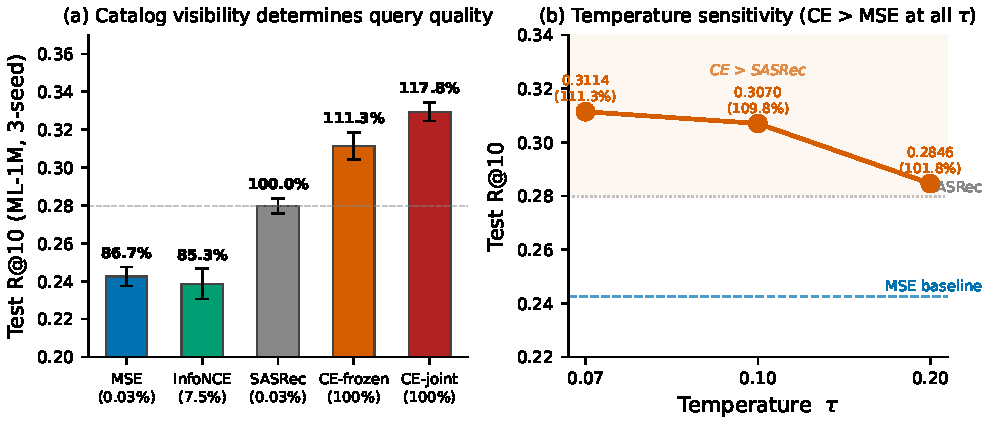
\includegraphics[width=0.92\columnwidth]{Figures/fig5_ce_mse.pdf}
\caption{Auxiliary objective and item-space diagnostic on ML-1M. MSE,
InfoNCE, and full-catalog CE in Table~\ref{tab:loss} keep the SASRec item
embedding space frozen. CE-joint updates the item representations and is shown
only as a separate diagnostic, not as a controlled loss-only comparison.}
\label{fig:ce-mse}
\end{figure}

\subsection{Temperature Ablation}
\label{app:temperature}

\begin{table}[!htbp]
\centering
\small
\begin{tabular}{lr}
\toprule
Objective & Test R@10 \\
\midrule
CQG-Single CE, $\tau=0.07$ & 0.3114 \\
CQG-Single CE, $\tau=0.10$ & 0.3070 \\
CQG-Single CE, $\tau=0.20$ & 0.2846 \\
CQG-Single MSE & 0.2425 \\
CQG-AR CE, $\tau=0.07$ & 0.2972 \\
CQG-AR CE, $\tau=0.10$ & 0.2886 \\
CQG-AR CE, $\tau=0.20$ & 0.2725 \\
\bottomrule
\end{tabular}
\caption{Temperature ablation on ML-1M under the corrected test-history
protocol. CQG-Single values are three-seed means; CQG-AR values are aligned
seed-42 controls. Lower temperatures improve shallow retrieval in the tested
range.}
\label{tab:temperature}
\end{table}

\section{LLM Backbone Diagnostic}
\label{app:llm}

We tested whether a pretrained LLM backbone improves continuous query
generation. Multiple Qwen configurations across three paradigms produced a
negative but informative result (Figure~\ref{fig:llm_diagnostic}). Shared
dual-tower training collapsed item representations, with item--item cosine
similarity increasing toward 0.9936. A frozen-item hybrid avoided item
collapse but produced loss--metric decoupling: InfoNCE loss improved while
Recall@10 remained far below the SASRec gate. The best text-aware hybrid
reached R@10 = 0.2118 on ML-1M but still trailed the single-run, MSE-frozen
scratch Transformer used in this diagnostic (R@10 = 0.248). This checkpoint
is distinct from the MSE-trained CQG-Single three-seed result of 0.2425 in
Table~\ref{tab:loss}.
This result does not imply that LLMs cannot support recommendation; it shows
that pretrained language representations are not automatically aligned with
the frozen collaborative item space.

\begin{figure}[!htbp]
\centering
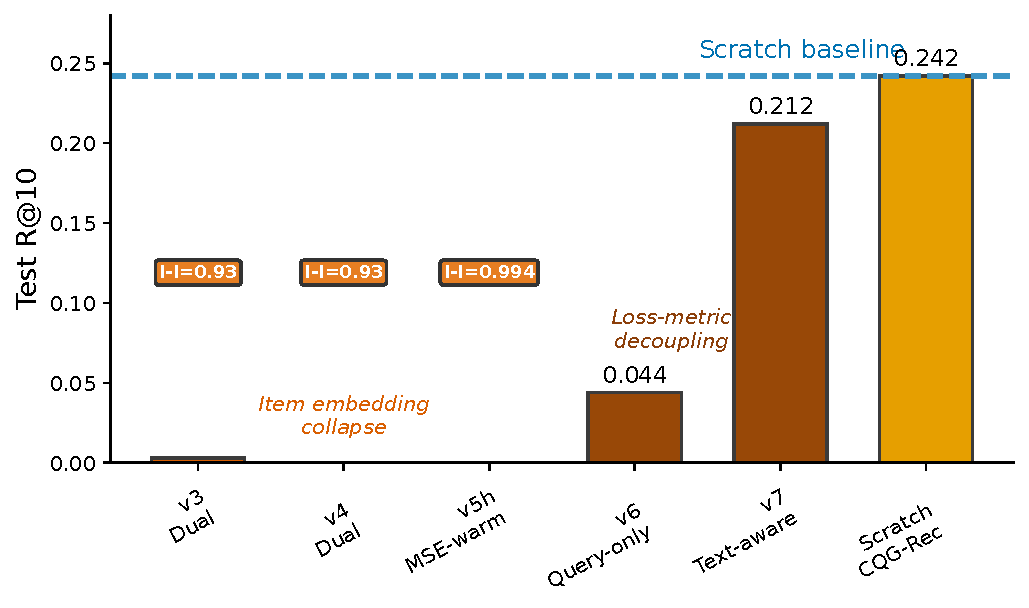
\includegraphics[width=0.72\textwidth]{Figures/fig4_llm_diagnostic.pdf}
\caption{LLM backbone diagnostics. Pretrained language backbones do not
automatically align with the frozen collaborative item space; the best
text-aware Qwen hybrid still trails the single-run, MSE-frozen scratch query
Transformer used in this diagnostic (R@10 = 0.248). This checkpoint is
separate from the three-seed CQG-Single MSE result in
Table~\ref{tab:loss}.}
\label{fig:llm_diagnostic}
\end{figure}

\begin{table}[!htbp]
\centering
\small
\begin{tabular}{lrrrrrr}
\toprule
Model & R@5 & R@10 & R@20 & R@50 & R@70 & R@90 \\
\midrule
\shortstack[l]{Scratch Transformer\\(LLM diagnostic)} & 0.172 & 0.248 & 0.345 & 0.498 & 0.555 & 0.595 \\
Qwen text-aware hybrid & 0.134 & 0.212 & 0.308 & 0.460 & 0.517 & 0.564 \\
\bottomrule
\end{tabular}
\caption{Single-run recall curve comparison between the MSE-frozen scratch
Transformer used in the LLM diagnostic and the best tested LLM hybrid
configuration. The scratch row is not the three-seed CQG-Single MSE aggregate
reported in Table~\ref{tab:loss}.}
\label{tab:llmcurve}
\end{table}

The full recall curve confirms the diagnostic: the best tested LLM hybrid
underperforms the scratch Transformer at every reported depth.

\section{Tokenization Diagnostics}
\label{app:tokenization}

Several neural RQ-VAE configurations collapsed to degenerate codebooks with
less than 10\% utilization. A k-means fallback achieved high code utilization
but showed large downstream variance across decoder configurations. We do not
use these failures as evidence that SID methods are generally weak; instead,
they motivate careful baseline validation against published TIGER, LETTER,
and EAGER results.

\begin{table}[H]
\centering
\small
\begin{tabular}{lll}
\toprule
Configuration & Utilization & Outcome \\
\midrule
Neural RQ-VAE variants & \(<\)10\% & Codebook collapse \\
k-means fallback A & 99.8\% & R@10 = 0.1230, 15\% reachability \\
k-means fallback B & 99.8\% & R@10 = 0.1932, 52\% reachability \\
\bottomrule
\end{tabular}
\caption{Tokenization diagnostics. Neural RQ-VAE collapsed in the tested configurations; k-means improved utilization but remained sensitive to decoder training and beam-search support.}
\label{tab:tokenization}
\end{table}

\section{Dynamic Catalog Discussion}
\label{app:dynamic}

CQG-Single and CQG-AR share the same index-level update interface. A new encoded item can be inserted into the ANN index without adding an output token, rebuilding a code trie, or changing either model's output dimensionality. This interface property does not guarantee cold-item ranking quality. In contrast, a SID system must assign the new item to a code path; if the assignment changes the code distribution or causes collisions, the codebook, trie, and decoder may need to be refreshed. A direct dynamic-catalog evaluation would hold out a fraction of items during training, insert them into the retrieval index only at test time, and measure new-item Recall@$K$, warm-item Recall@$K$, index update cost, and whether model retraining is required.
